\section{extendedTerm - WIP}
(sloppily copied from 200806-ExtendedVersionComp)

\subsection{Scenario - WIP} 
\begin{itemize}
\footnotesize
\raggedright
\singlespacing
\itemsep 0em
\item Kundur  4 machine system packaged with PST - Same as used in AGC examples...
\item Constant Z load model
\item System has governors, exciters, and PSS.
\item Governor of generator being perturbed by pm\_sig removed
\item Perturbance was meant to mimic a solar ramp with various situations of cloud cover:\\
\begin{Verbatim}[fontsize=\scriptsize]
% time [seconds]
% 0-30      - no action
% 30-90     - ramp up 0.5 PU (50 MW)
% 90-150    - hold peak
% 150-210   - ramp down 0.5 PU (50 MW)
% 210-240   - no action

% cloud cover events
% 45-55 - 20% max gen (generation of 0.1 PU)
% 120-140 - 30% cover (generation reduction to 70%)
% 180-190 - 15% cover (generation reduction to 85%)
\end{Verbatim}
\end{itemize}


\begin{figure}[H]
	\centering
	\footnotesize
	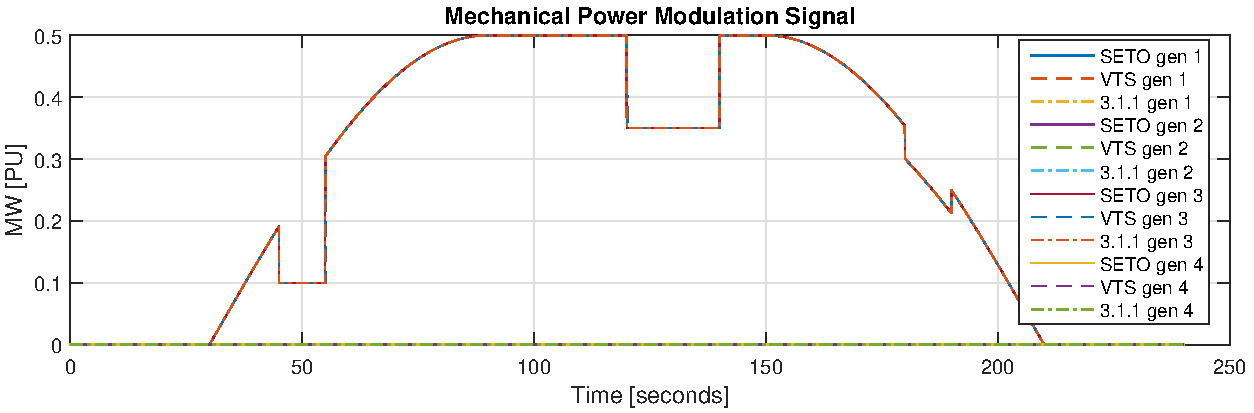
\includegraphics[width=\linewidth]{examples/extendedTerm/extended-1}
	\caption{Modulation signal extended example.}
	\label{fig: extended 1}
\end{figure}%\vspace{-1 em}




\pagebreak
\subsection{Result Summary - WIP} 
\begin{enumerate}
\itemsep 0 em
\item PST 4 is 2.6 times faster than PST 3.1.
\item Using variable time steps allows for a speed up of 5.9 over PST 3.1.
\item Results from all simulations are very similar.
\item Without creating an explicit time block at the beginning of an event, VTS events may not occur at the exact time they are programmed.
\item VTS reduces logged data size by $\approx$3 times.
\end{enumerate}


\begin{table}[!ht]
\resizebox{\linewidth}{!}{

	\begin{tabular}{@{} L{1.75cm} 
	R{2cm} R{2cm}  R{2cm} R{1.5cm} R{0.75cm} R{0.75cm} R{1.5cm} R{2cm} R{2cm}@{}} 	
		\toprule % @ signs to remove extra L R space
		\footnotesize % this will affect the table font (makse it 10pt)
		\raggedright % for non justified table text

	&	\multicolumn{3}{c}{Step Size [seconds]}					&		&	\multicolumn{2}{c}{Solutions Per Step}			&		&		&		\\	
\shortstack{PST\\Version}	&	Max.	&	Min.	&	Ave.	&	Total Steps	&	Ave.	&	Max.	&	Total Slns.	&	Sim. Time	&	Speed Up	\\ \midrule	

3.1	&	4.00E-03	&	4.00E-03	&	4.00E-03	&	59,975	&	2	&	2	&	119,950	&	740.35	&	1.00	\\
SETO	&	4.00E-03	&	4.00E-03	&	4.00E-03	&	59,975	&	2	&	2	&	119,950	&	284.37	&	2.60	\\
4.0 - VTS	&	23.2	&	1.36E-04	&	1.38E-02	&	17,353	&	2	&	96	&	27,243	&	125.53	&	5.90	\\


																				\bottomrule
	\end{tabular}
	}%end resize box
		\caption{PST Version Comparisons of Extended Term Example.}
		\label{tab: extended}


\end{table}


\begin{figure}[H]
	\centering
	\footnotesize
	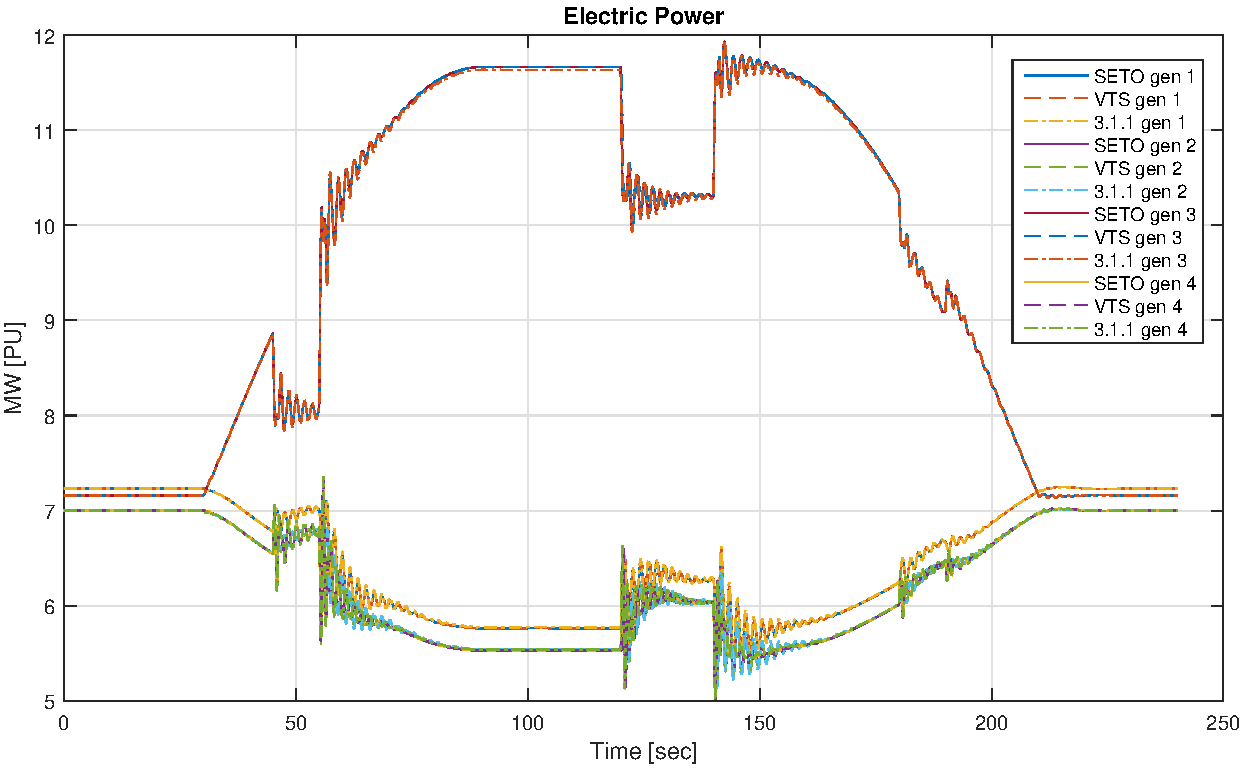
\includegraphics[width=\linewidth]{examples/extendedTerm/extended-7}
	\caption{Electric Power from extended example.}
	\label{fig: extended 7}
\end{figure}%\vspace{-1 em}


\pagebreak
% fixed: 8749 steps i.e., 17498 network solutions 

%>> compareVTSandFTS
%VTS time: 15.8579
%fixed time: 57.4479
NOTE: Initial time steps before t=30 are much larger than the other time steps (multiple seconds) and are plotted off the axis.

\begin{figure}[H]
	\centering
	\footnotesize
	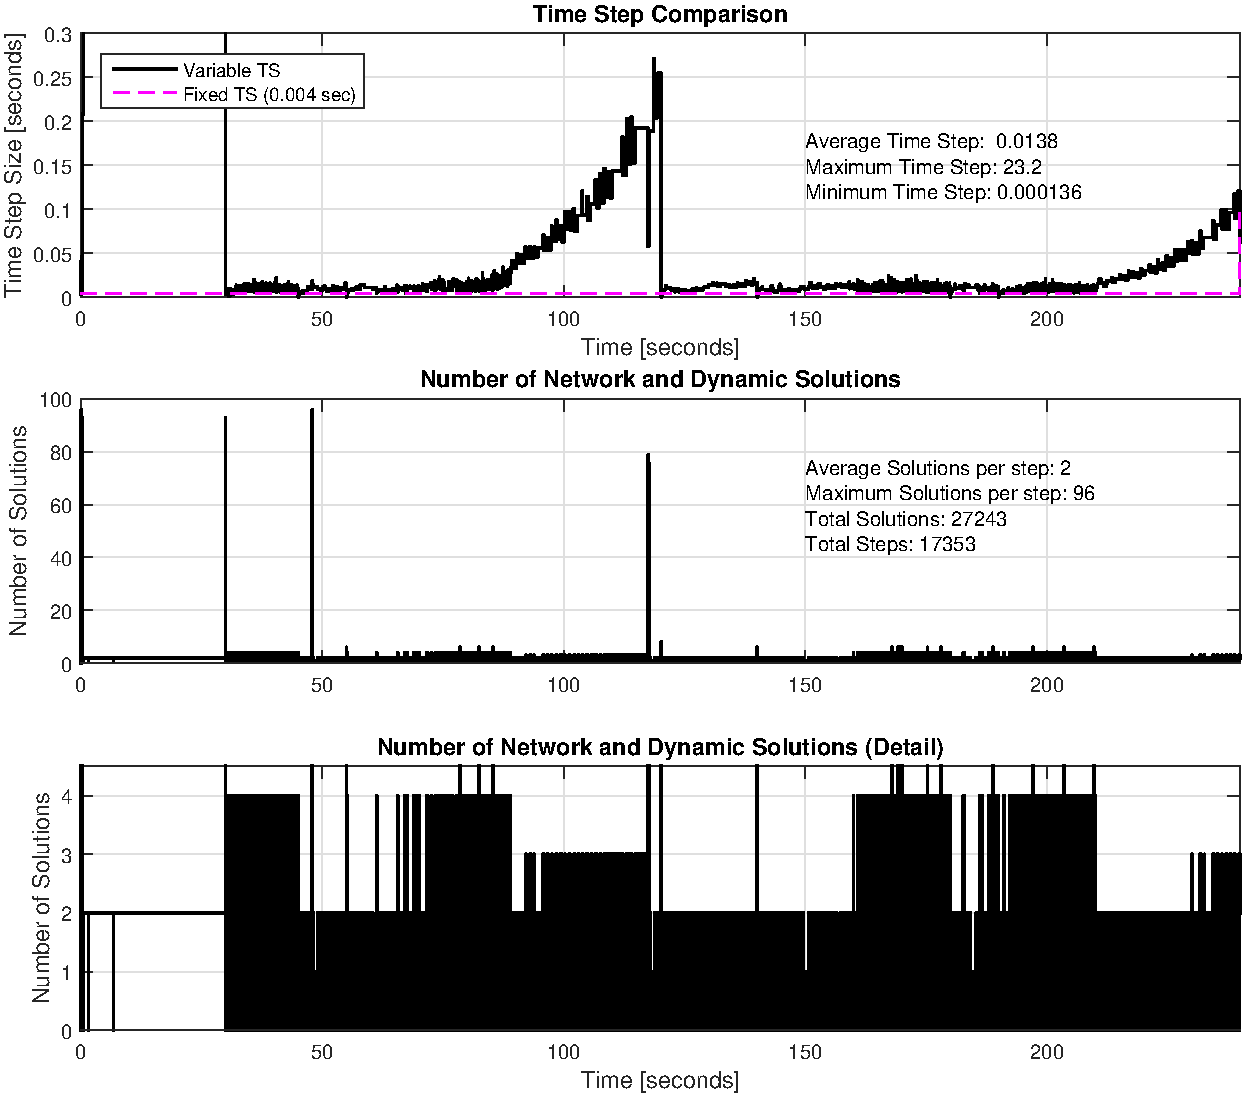
\includegraphics[width=\linewidth]{examples/extendedTerm/extended-2}
	\caption{Step Size / Number of Solutions Comparison extended.}
	\label{fig: extended 2}
\end{figure}%\vspace{-1 em}




\pagebreak
NOTE: 3.1 does not calculate average system frequency.
\begin{figure}[H]
	\centering
	\footnotesize
	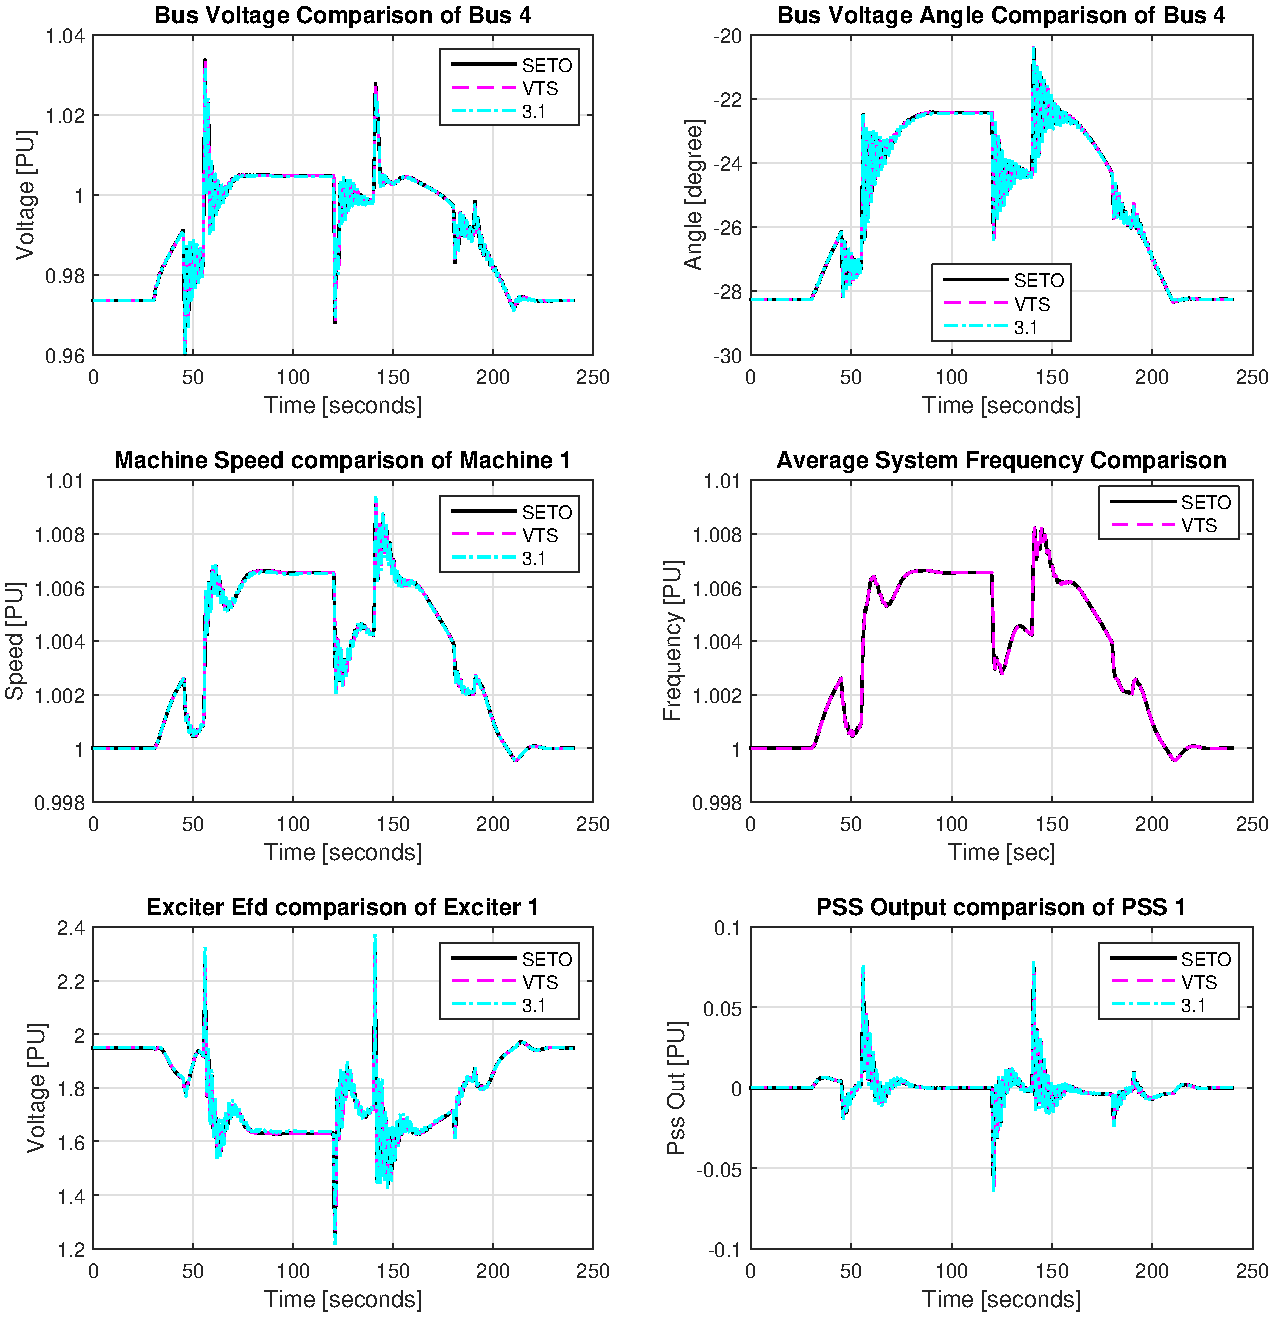
\includegraphics[width=\linewidth]{examples/extendedTerm/extended-3}
	\caption{Various Comparisons extended.}
	\label{fig: extended 3}
\end{figure}%\vspace{-1 em}

\pagebreak

NOTE: PST 3.1 uses the \verb|pss3| model while other PST versions use \verb|pss2|
\begin{figure}[H]
	\centering
	\footnotesize
	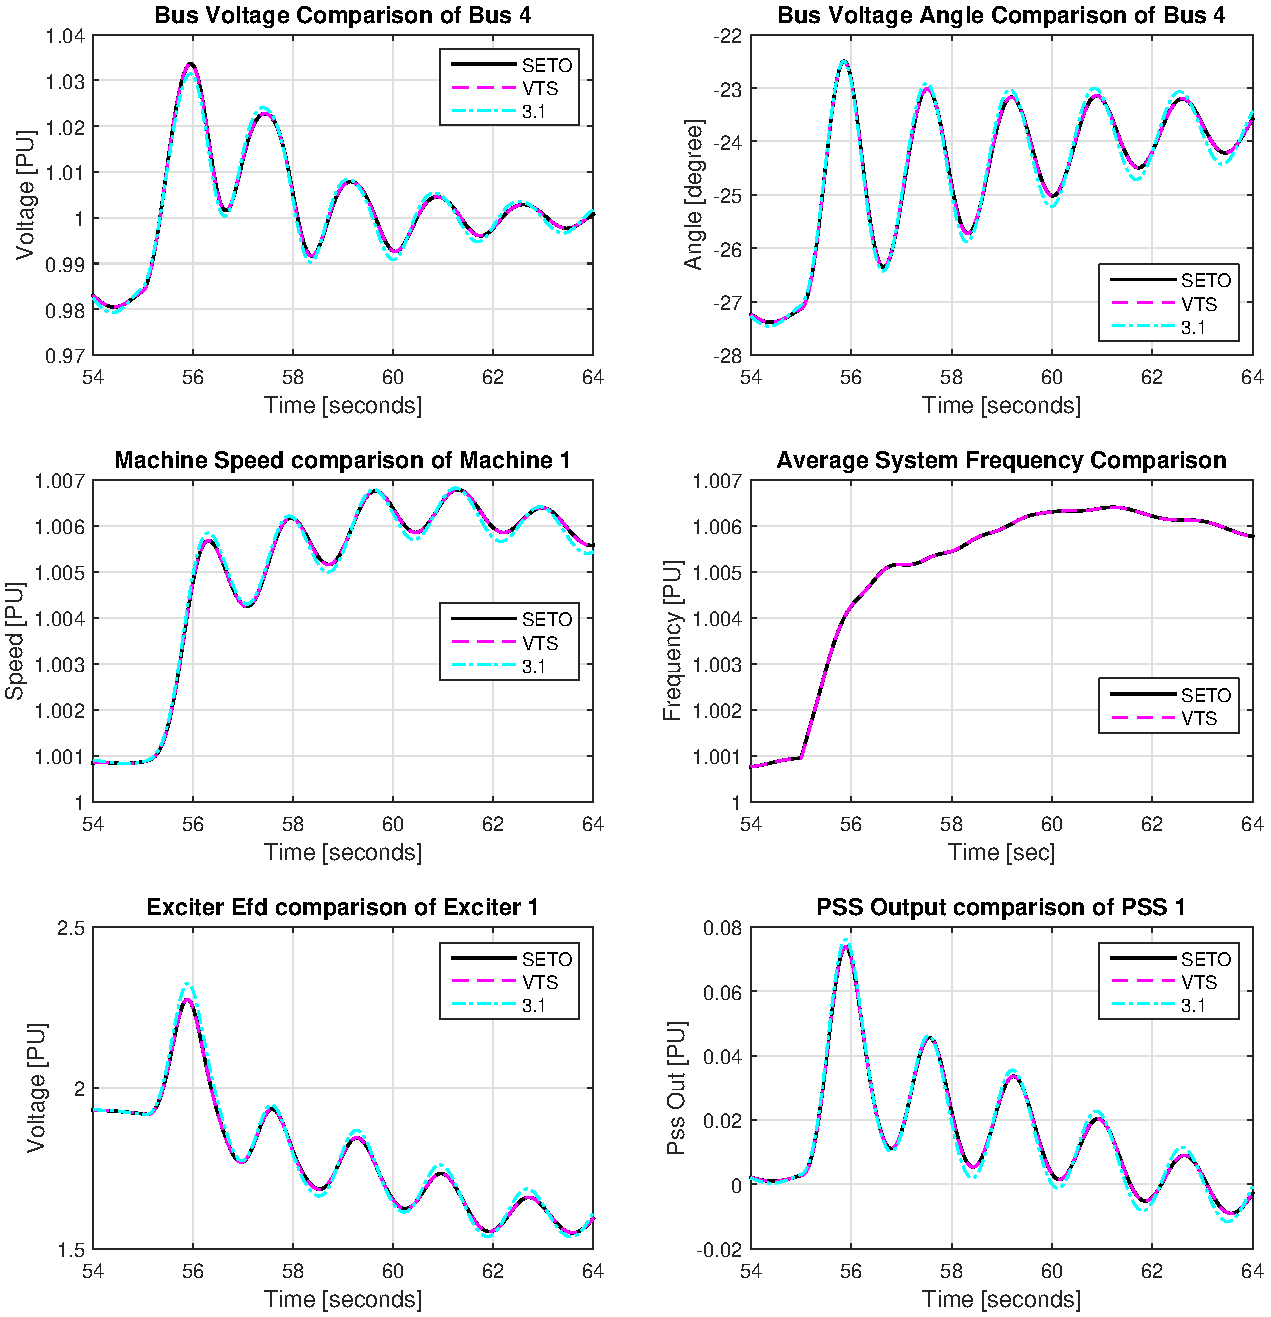
\includegraphics[width=\linewidth]{examples/extendedTerm/extended-4}
	\caption{Various Comparisons - Detail 1 extended.}
	\label{fig: extended 4}
\end{figure}%\vspace{-1 em}

\pagebreak

\begin{figure}[H]
	\centering
	\footnotesize
	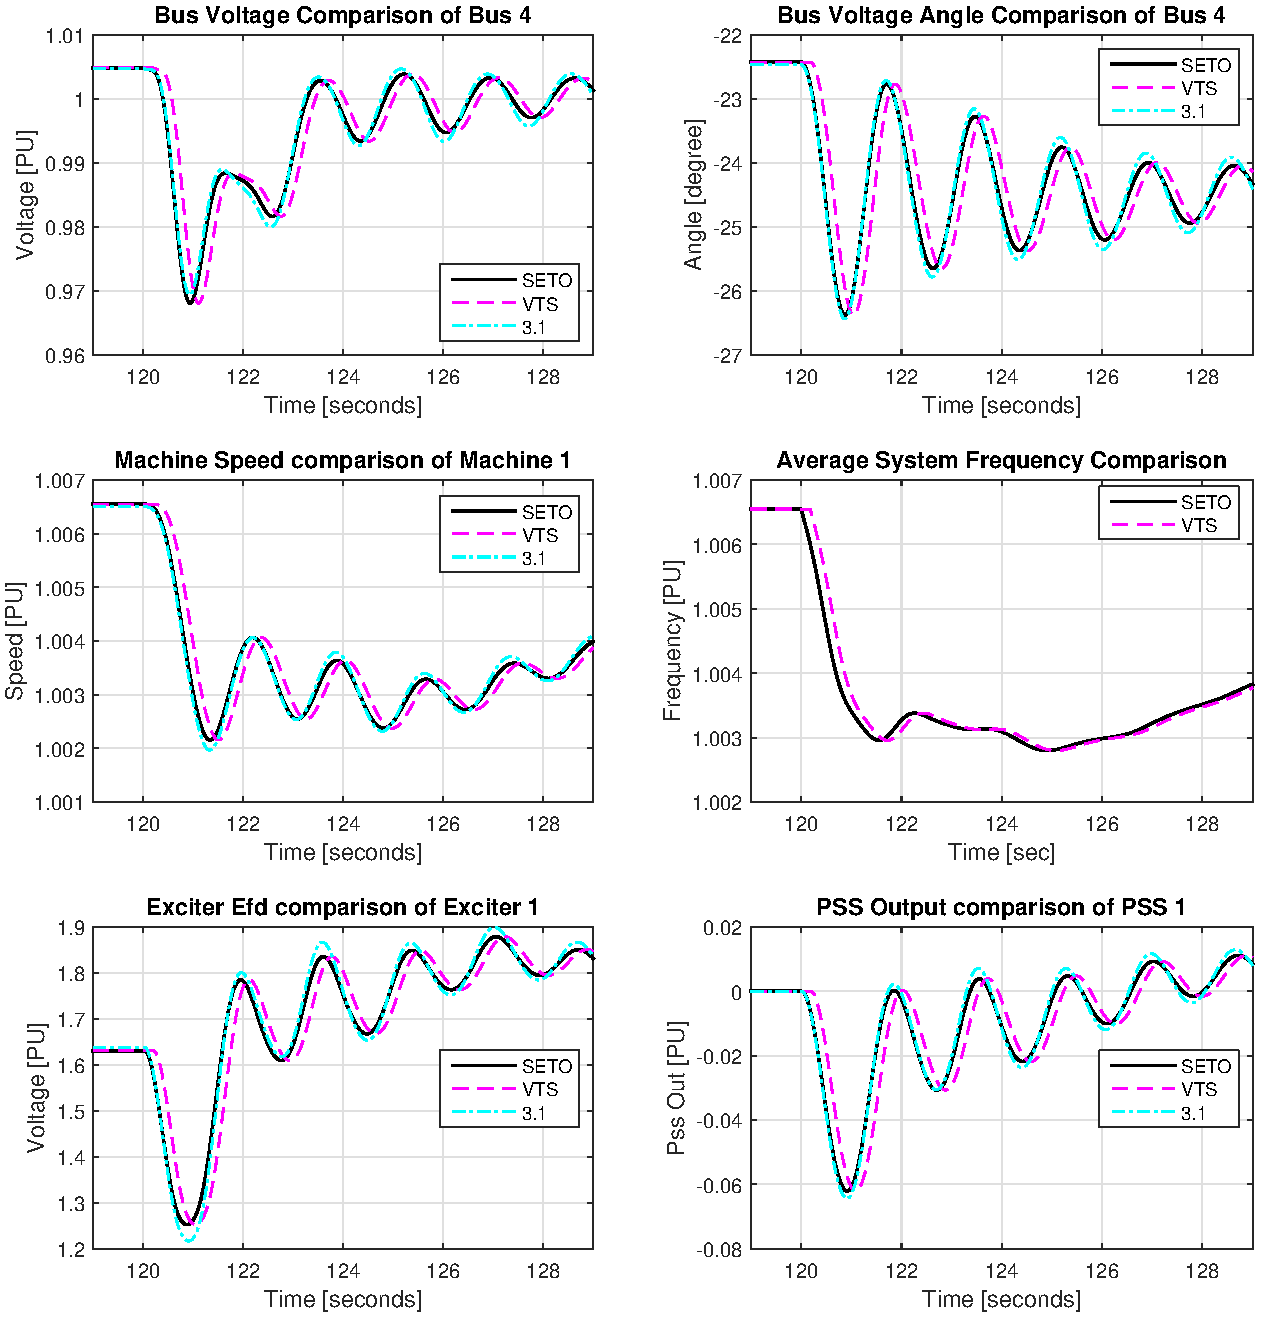
\includegraphics[width=\linewidth]{examples/extendedTerm/extended-5}
	\caption{Various Comparisons - Detail 2 extended.}
	\label{fig: extended 5}
\end{figure}%\vspace{-1 em}

Figure \ref{fig: extended 5} NOTE: VTS events may not occur at exact specified time due to the nature of variable time steps.
Additional entries in the \verb|sw_con| can be created to account for this.
For example, creating an entry for every known perturbance can ensure the exact execution time.


\pagebreak

\begin{figure}[H]
	\centering
	\footnotesize
	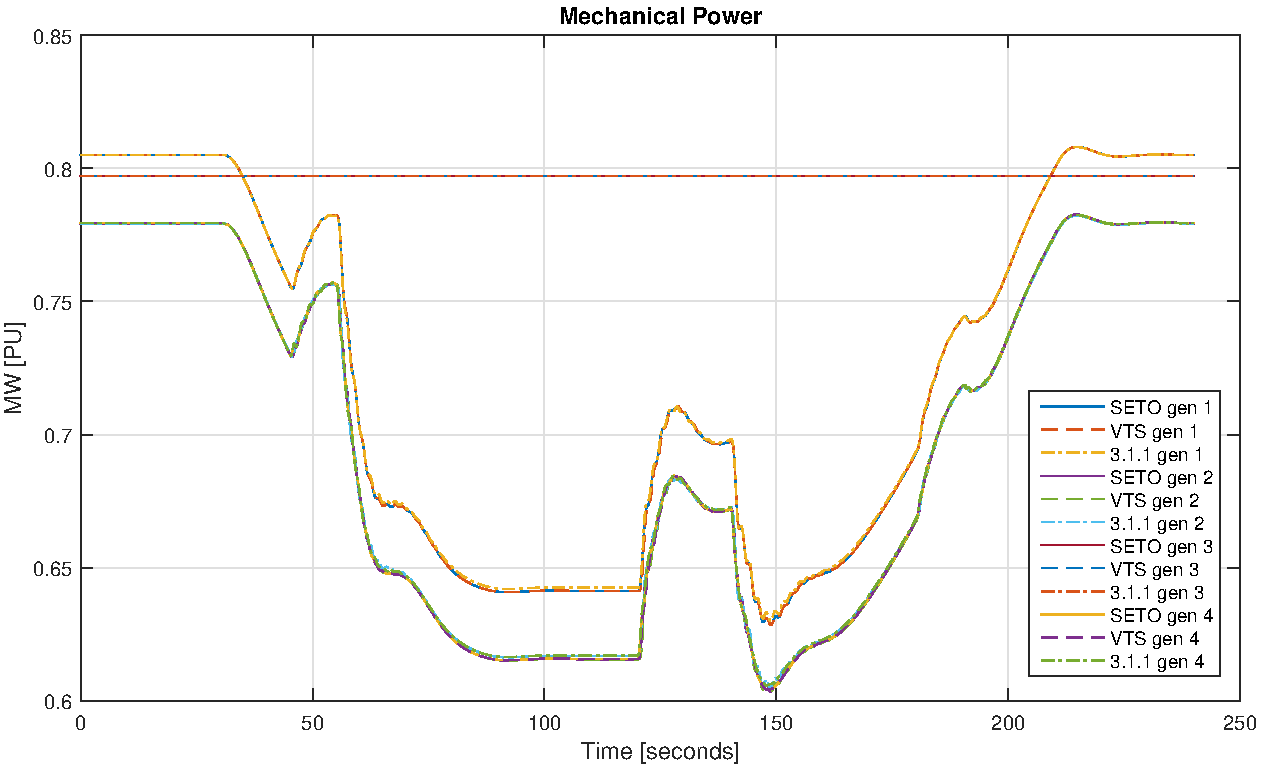
\includegraphics[width=\linewidth]{examples/extendedTerm/extended-6}
	\caption{Mechanical Power extended.}
	\label{fig: extended 6}
\end{figure}%\vspace{-1 em}

PST does not add the modulated mechanical power signal the recorded mechanical power.
Instead, the modulation signal is added to the derivative of machine speed.



